\section{Methods}

\subsection{Sparsification}

Each coarse matrix is computed by the triple product $As[l+1] = R[l] \times As[l] \times P[l]$, then it is sparsified
based on a randomized strategy. We want to retain the majority of entries with higher absolute values and also
a few entries with lower absolute values. The element-wise matrix sparsification suggested in [] is not efficient in practice.



Algorithm \ref{alg:spars001} shows an improved version.
Matrix $A$ is saved as a vector of entries with an arbitrary order.
The probability of selecting each entry $A_{ij}$  is

\begin{equation}
 p_{ij} = \frac{A_{ij}^2}{\sum_{lk} A_{lk}^2}
\end{equation}
in which the summation goes through all entries of $A$ (Frobenius norm of $A$).

\begin{algorithm}[H] 
  \footnotesize
  \caption{$As = Sparsify(A, S, F)$} \label{alg:spars001} 
  \begin{algorithmic}[1]
    \Require $A$ (original matrix), $S$ (size of the sparsified matrix), $F$ (Frobenius norm of $A$)
    \Ensure  $As$ (sparsified matrix)
    \State $iter \leftarrow 0$, $i \leftarrow 0$
    \While{$i < S$}
    
      \State $p_{iter} \leftarrow \frac{A[iter]^2}{F}$ \Comment{probability of entry $iter$}
      
      \If{$rand() < p_{iter}$}
	\State $As \leftarrow A[iter]$
	\State $i++$
      \EndIf
      
      \State $iter++$
      \If{$iter \geq size(A)$}
	\State $iter -= size(A)$
      \EndIf
      
    \EndWhile
  \end{algorithmic}
\end{algorithm}

The issue with Algorithm \ref{alg:spars001} is that for big matrices, the probability of choosing each entry becomes very low,
because the denominator becomes very large, relative to the numerator (check first line in Figure~\ref{fig:spars001}).

To fix this issue, the probability of each entry is scaled to the whole $[0,1]$ interval by multiplying all the probabilities
by the highest probability (second and third lines in Figure~\ref{fig:spars001}). Algorithm \ref{alg:spars002} shows
how the probabilities are scaled.

\begin{figure}[tbh]
 \centering
 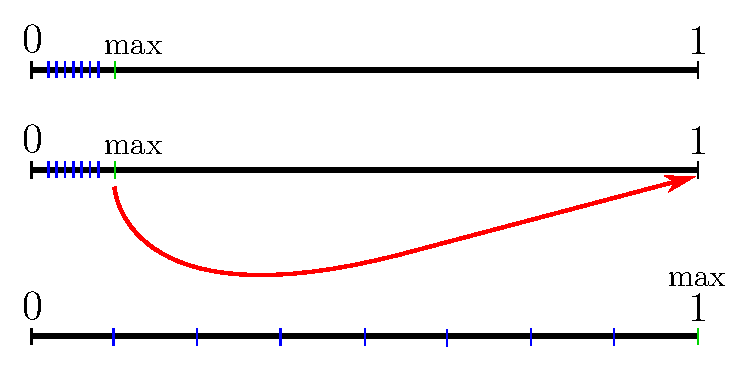
\includegraphics[width=7cm,height=4cm]{./figures/spars001.pdf}
 \caption{Scaling the probabilities of choosing entries to be retained, to the unit interval}
 \label{fig:spars001}
\end{figure}

\begin{algorithm}[H] 
  \footnotesize
  \caption{$As = Sparsify(A, S, F, max)$} \label{alg:spars002} 
  \begin{algorithmic}[1]
    \Require $A$ (original matrix), $S$ (size of the sparsified matrix), $F$ (Frobenius norm of $A$), $max$ (maximum value of $A$) 
    \Ensure  $As$ (sparsified matrix)
    \State $iter \leftarrow 0$, $i \leftarrow 0$
    \State $IMP = \frac{F}{max^2}$ \Comment{$IMP$: inverse of max probability}
    \While{$i < S$}
    
      \State $p_{iter} \leftarrow \frac{IMP * A[iter]^2}{F}$ \Comment{probability of entry $iter$}
      
      \If{$rand() < p_{iter}$}
	\State $As \leftarrow A[iter]$
	\State $i++$
      \EndIf
      
      \State $iter++$
      \If{$iter \geq size(A)$}
	\State $iter -= size(A)$
      \EndIf
      
    \EndWhile
  \end{algorithmic}
\end{algorithm}

This algorithm may take a long time, since the random value is generated in the unit interval $[0,1]$,
and some entries may still have very low absolute value and consequently very low probability.  
To fix that, after passing through all the entries of the matrix once, the random value will be generated in a tenth
of the unit interval $[0,0.1]$ for the next round and between $0$ and $0.01$ for the round after
that and so on (Algorithm \ref{alg:spars003}).

\begin{algorithm}[H] 
  \footnotesize
  \caption{$As = Sparsify(A, S, F, max)$} \label{alg:spars003} 
  \begin{algorithmic}[1]
    \Require $A$ (original matrix), $S$ (size of the sparsified matrix), $F$ (Frobenius norm of $A$), $max$ (maximum value of $A$) 
    \Ensure  $As$ (sparsified matrix)
    \State $iter \leftarrow 0$, $i \leftarrow 0$, $randFactor \leftarrow 1$ \Comment{initialize $randFactor$ to $1$}
    \State $IMP = \frac{F}{max^2}$
    \While{$i < S$}
    
      \State $p_{iter} \leftarrow \frac{IMP * A[iter]^2}{F}$
      
      \If{$rand() / randFactor < p_{iter}$}
	\State $As \leftarrow A[iter]$
	\State $i++$
      \EndIf
      
      \State $iter++$
      \If{$iter \geq size(A)$}
	\State $iter -= size(A)$
	\State $randFactor *= 10$
      \EndIf
      
    \EndWhile
  \end{algorithmic}
\end{algorithm}

We want the matrix to stay symmetric after sparsification. Also, the diagonal entries should be kept (why? smoothers?).
So we go through the lower triangle of the matrix. We add every diagonal entry. And if a non-diagonal entry is 
chosen to be added, its transpose entry will be added too. Also a boolean vector is used to avoid having duplicates.
This way we will have a matrix of exactly the desired size and also there is no need to remove duplicates
(Algorithm \ref{alg:spars004}).

\begin{algorithm}[H] 
  \footnotesize
  \caption{$As = Sparsify(A, S, F, max)$} \label{alg:spars004} 
  \begin{algorithmic}[1]
    \Require $A$ (original matrix), $S$ (size of the sparsified matrix), $F$ (Frobenius norm of $A$), $max$ (maximum value of $A$) 
    \Ensure  $As$ (sparsified matrix)
    \State $i \leftarrow 0$
    \State $chosen[size(A)] \leftarrow False$ \Comment{initialize boolean vector to $False$}
    
    \For{$iter=0;\ iter<nnz, i<S;\ iter++$}
      \If{$A[iter].row == A[iter].col$}
	    \State $As \leftarrow A[iter]$
	    \State $chosen[iter] \leftarrow True$
	    \State $i++$
      \EndIf
	
    \EndFor
    \State $iter \leftarrow 0$, $randFactor \leftarrow 1$ \Comment{initialize $randFactor$ to $1$}
    \State $IMP = \frac{F}{max^2}$
    \While{$i < S$}
    
      \If{$!chosen[iter]$ and $A[iter].row < A[iter].col$}
    
	\State $p_{iter} \leftarrow \frac{IMP * A[iter]^2}{F}$
	
	\If{$rand() / randFactor < p_{iter}$}
	
	  \State $As \leftarrow A[iter]$
	  \State $As \leftarrow A[iter]^T$
	  \State $i += 2$

	    \State $chosen[iter] \leftarrow True$
	\EndIf
      
      \EndIf
      
      \State $iter++$
      \If{$iter \geq size(A)$}
	\State $iter -= size(A)$
	\State $randFactor *= 10$
      \EndIf
      
    \EndWhile
  \end{algorithmic}
\end{algorithm}


